%\vspace{-10pt}

\section{Introduction} \label{sec:intro}

%\vspace{-4pt}

\begin{figure*}[!t]
\centering
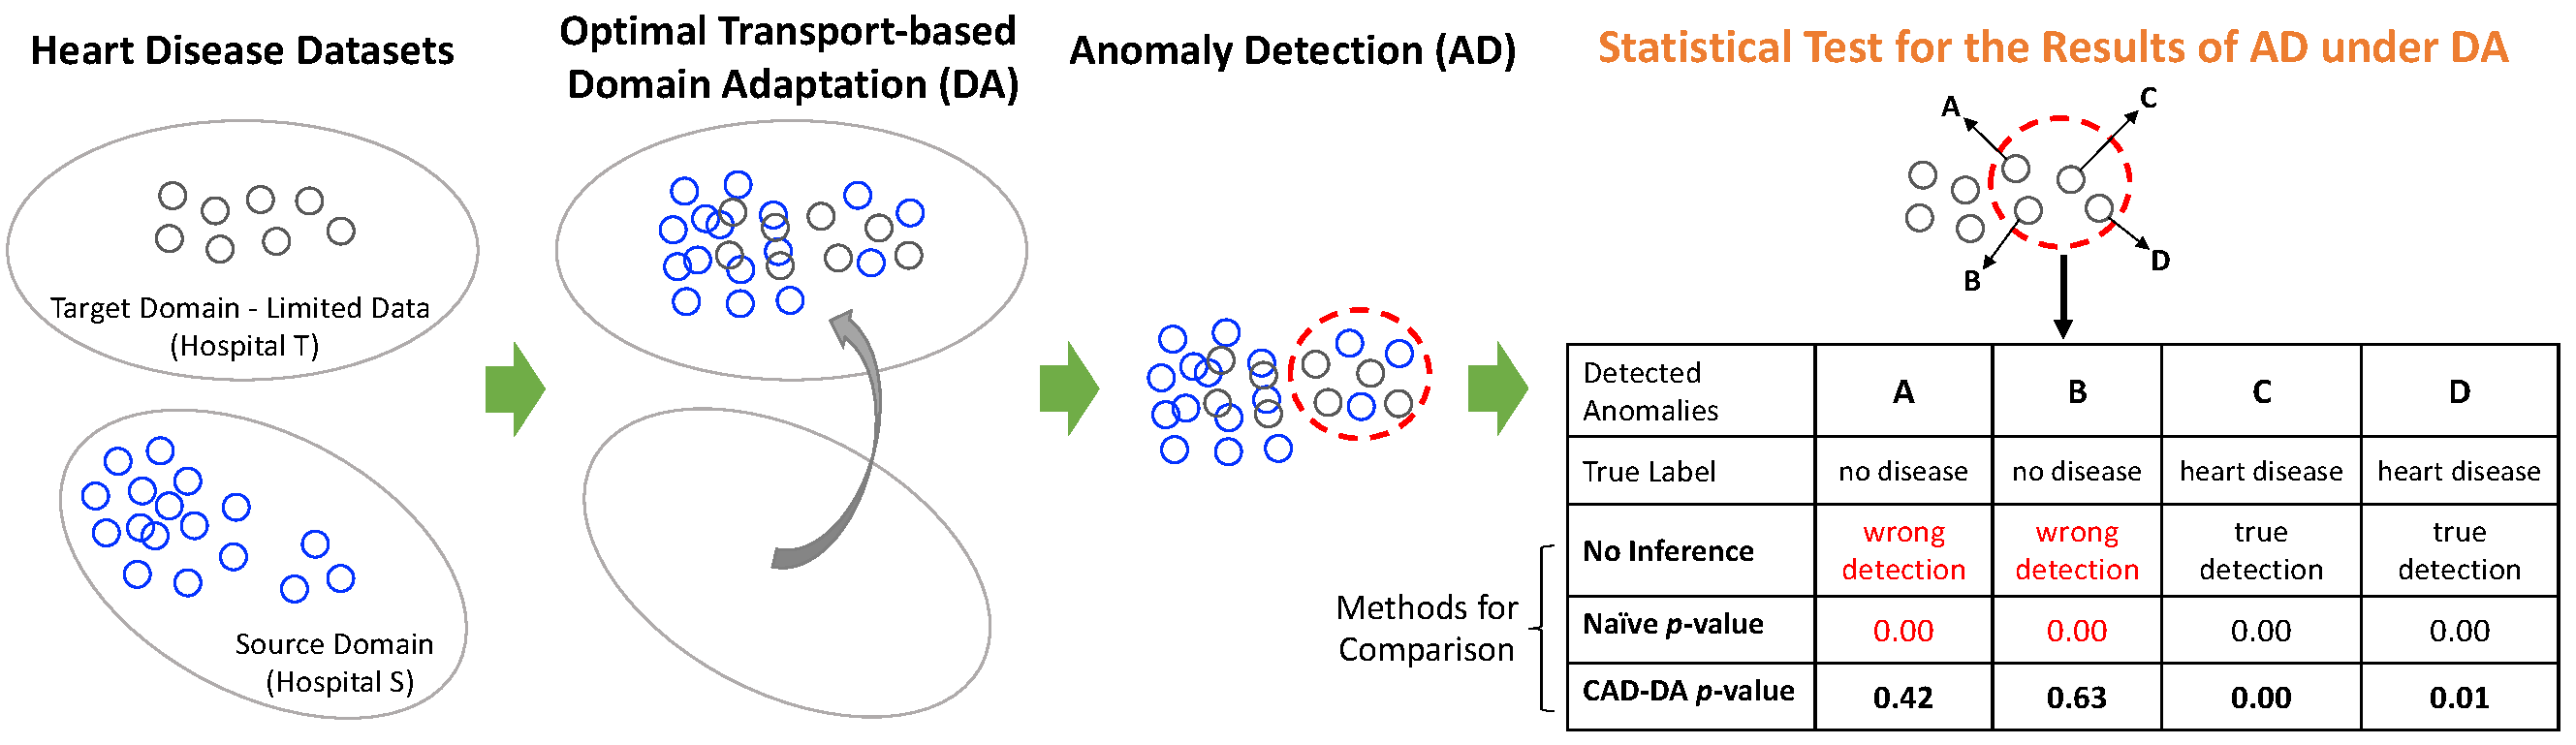
\includegraphics[width=.85\textwidth]{demo.pdf}
%\vspace{-4pt}
\caption{Illustration of the proposed method.
%
Conducting AD-DA without inference results wrong anomalies (\textbf{A}, \textbf{B}).
%
The naive $p$-values are small even for falsely detected anomalies.
%
The proposed CAD-DA can identify both false positive (FP) and true positive (TP) detections, i.e., large $p$-values for FPs and small $p$-values for TPs.
}
\label{fig:illustration}
\vspace{-5pt}
\end{figure*}

%\htcomment{
%suggested re-writing (condensing)\\
%===\\
%
%Anomaly detection (AD) is a fundamental problem in machine learning and statistics, as the vast body of literature surveyed by Aggarwal~\cite{aggarwal2017outlier} suggests.
%The goal of AD is to identify rare and unusual observations that deviate significantly from the norm within a given dataset.
%AD plays a critical role in several applications and has been widely applied in many areas such as medical \cite{wong2002rule, aggarwal2005abnormality}, fraud detection \cite{pourhabibi2020fraud}, and damage detection \cite{avci2021review, du2020damage}.
%}

Anomaly detection (AD) is a fundamental problem in machine learning and statistics, as the vast body of literature surveyed by \cite{aggarwal2017outlier} suggests.
%
% \htcomment{
% maybe say "a fundamental problem in statistics and machine learning"
%
% \red{Duy: updated}
% }
% \htcomment{add a few citations to justify ``many areas''
%
% \red{Duy: updated}}
% \htcomment{``studied'' sounds weak, may consider using some more concrete terms---do we mean applicable to many areas or what?
%
% \red{Duy: updated}}
%
The goal of AD is to identify rare and unusual observations that deviate significantly from the norm within a given dataset.
AD plays a critical role in several applications and has been widely applied in many areas such as medical \cite{wong2002rule, aggarwal2005abnormality}, fraud detection \cite{pourhabibi2020fraud}, and damage detection \cite{avci2021review, du2020damage}.


In numerous real-world scenarios, the availability of limited data can lead to poor performance of AD. 
%
To overcome this challenge, a strategy of increasing the sample size by transferring data points from a readily accessible source domain to the present target domain can be employed. 
%
This type of problem is known as Domain Adaptation (DA).
%
By leveraging data-rich source domains to bolster the data pool in the target domain, DA aims to enhance the efficacy of AD in scenarios where limited data hamper their effectiveness.



A critical concern arises regarding to the possibility of erroneous detection.
% when conducting AD after DA.  
%
The AD could misidentify certain observations as anomalies, even though they are actually normal. 
%
These errors are commonly referred to as \emph{false positives},
%
%The false positives 
which can cause serious consequences in high-stake decision making.
%when they are used for high-stake decision making.
%The utilization of the false positives can cause serious consequences, particularly in applications with critical decision-making stakes.
%, such as medical diagnosis or treatment recommendations. 
%
%Especially, when conducting AD based on samples obtained by DA, there is a higher chance of misclassifying normal instances as anomalies, due to potential errors in the DA process.
Especially, when conducting AD under DA, there is an increased risk of misclassifying normal instances as anomalies due to potential DA errors.
%
%based on samples obtained by DA, there is a higher chance of misclassifying normal instances as anomalies, due to potential errors in the DA process.
%
For instance, in the medical field, some unhealthy individuals transformed from the source domain may become closely similar to healthy individuals in the target domain.
%
Thus, we mistakenly classify a healthy individual as unhealthy, and we could inadvertently administer drugs that may harm their well-being. 
%
%Patients may become apprehensive about seeking medical help, fearing misdiagnosis and unnecessary treatments.
%
%Similarly, in cybersecurity, incorrect identification of cyberattacks wastes resources, and causes financial losses.
%
Hence, there is a critical need of an inference method  for controlling the false positive rate (FPR).
% in high-stakes decision-making scenarios.


In AD-DA, controlling the false negative rate (FNR) is also important.
%, and it involves a trade-off with the FPR.
%
In the literature of statistics, a common procedure is to initially control the FPR at a specified level $\alpha$, e.g., 0.05, while concurrently seeking to minimize the FNR, i.e., maximizing the true positive rate (${\rm TPR} = 1 - {\rm FNR}$)
%, where ${\rm TPR} = 1 - {\rm FNR}$, 
by empirical evidences.
%
In this paper, we also follow this established practice.
%
We propose a method to theoretically control the probability of misidentifying a normal observation as an anomaly while endeavoring to minimize the probability of misidentifying an anomaly as normal.




To our knowledge, none of the existing method can control the FPR of AD under the context of DA.
%
The main challenge is that, without accounting for the influence of DA, the FPR can not be properly controlled.
%
%The major difficulty of this setting is that the DA, AD, and inference are conducted on the same data.
%%
%Traditional statistical inference, which assumes that the target of inference must be fixed a priori or obtained from independent dataset, cannot be used for this problem.
%
The authors of \cite{tsukurimichi2022conditional} proposed a method for testing the anomalies when they are detected by a class of robust regression methods \cite{huber1973robust, andrews1974robust, zaman2001econometric, rousseeuw2005robust, maronna2019robust}.
%, based on the concept of conditional Selective Inference \cite{lee2016exact}.
%
However, this method supposes that the data comes from the same distribution, and it is invalid in the scenario that a distribution shift occurs and DA must be applied.



Our idea is to leverage \emph{Selective Inference (SI)} \cite{lee2016exact} for resolving this challenge.
%
However, directly incorporating SI in our setting is still non-trivial because SI is highly \emph{problem-specific}.
%
Therefore, we need to carefully examine the selection strategy of the algorithm in the context of AD after DA.
%
Moreover, if we naively leverage the ideas of existing SI methods \cite{lee2016exact, duy2021exact}, the power of the test is significantly low, i.e, the FNR is high.
%
Therefore, we need to introduce an approach to minimize the FNR while properly controlling the FPR.
%
We would like to note that we start this new research direction with the Optimal Transport (OT)-based DA \cite{flamary2016optimal}, which is recently promising and popular in the OT community. The detailed discussions on future extensions to other types of DA are provided in \S \ref{sec:discussion}.

%\vspace{-5pt}

\paragraph{Contributions.} Our contributions are as follows:

$\bullet$ We mathematically formulate the problem of testing AD results under DA and introduce \emph{CAD-DA}, a novel method to conduct the statistical test with controllable FPR. 
%
Compared to the literature on controllable AD, CAD-DA presents a unique challenge in addressing the effect of DA to ensure the validity of FPR control.



$\bullet$ We overcome the challenge by leveraging the SI framework to handle the influence of DA.
%
We carefully examine the selection strategy for OT-based DA, whose operations can be characterized by linear/quadratic inequalities, and prove that achieving controllable AD-DA is indeed possible.
%
Furthermore, we introduce a more strategic approach to enhance the TPR.
%
To our knowledge, this is the first work capable of conducting valid inference within the context of DA.


%We propose a novel statistical inference method, named \emph{CAD-DA}, for testing the results of AD-DA with controllable FPR. 
%%
%Compared to the literature on controllable AD, CAD-DA presents a unique challenge in addressing the effect of DA to ensure the validity of the guarantee.
%%
%To our knowledge, this is the first method that can account the effect of DA and compute a valid $p$-value for the anomalies under DA setting.
%
%By using the proposed $p$-value, the FPR is theoretically controlled under a given significance level $\alpha$ (e.g., 0.05).


$\bullet$ We conduct experiments on both synthetic and real-world datasets to support our theoretical results, showcasing superior performance of the CAD-DA.

%\vspace{2pt}

\begin{example}
To show the importance of the proposed method, we provide an example presented in Fig. \ref{fig:illustration}.
%
Our goal is to detect patients in Hospital T with heart disease, treated as anomalies, in a scenario where the number of patients is limited.
%
Here, the source domain consists of patients in Hospital S, while the target domain comprises patients in Hospital T.
%
We employ the OT-based DA approach to transfer the data from the source domain to the target domain.
%
Subsequently, we apply an AD algorithm, i.e., mean absolute deviation.
%
The AD algorithm erroneously identified two healthy individuals as anomalies. 
%
To address this issue, we conducted an additional inference step using the proposed $p$-values, allowing us to identify both true positive and false positive detections.
%
Furthermore, we repeated the experiments $N$ times and the FPR results are shown in Tab. \ref{tbl:example_intro}.
%
With the proposed method, we were able to control the FPR under $\alpha = 0.05$, which other competitors were unable to achieve. 
\end{example}


\begin{table}[t]
\renewcommand{\arraystretch}{1.2}
\centering
\caption{The importance of the proposed method lies in its ability to control the False Positive Rate (FPR).}
\vspace{-5pt}
\begin{tabular}{ |l|c|c|c| } 
  \hline
  & \textbf{No Inference} & \textbf{Naive} & \textbf{CAD-DA} \\
  \hline
  $N = 120$ & FPR = 1.0 & 0.6 & \textbf{0.04} \\
   \hline
  $N = 240$ & FPR = 1.0 & 0.7 & \textbf{0.05} \\
  \hline
\end{tabular}
\label{tbl:example_intro}
\vspace{-10pt}
\end{table}



\textbf{Related works.}
Although there exists an extensive body of literature on AD methods \cite{aggarwal2017outlier}, there has been a limited exploration of applying the hypothesis testing framework to assess the results of AD. 
%
For instance, in \cite{srivastava1998outliers} and \cite{pan1995multiple}, the likelihood ratio test has been discussed to determine if an individual data point is an anomaly, employing the mean-shift model.
% --- a widely used model for characterizing the presence of anomalies.
%
However, these classical anomaly inference methods hold validity exclusively when the target anomalies are pre-determined in advance. 
%
When we employ these classical techniques on the anomalies detected by an AD algorithm, they become invalid in the sense that the FPR cannot be controlled at the desired level.


In order to control the FPR when using classical methods, the use of multiple testing correction is essential.
%
The most popular technique is Bonferroni correction, in which the correction factor scales exponentially with the number of instances, denoted as $n$. 
%
Specifically, it grows to a value of $2^n$.
%
However, this correction factor can become prohibitively large unless $n$ fairly small, which leads to overly conservative statistical inference.



In recent years, SI has emerged as a promising approach to resolve the invalidity of the traditional inference method without the need of employing conservative multiple testing correction. 
%
Specifically, instead of considering the exponentially increasing value of $2^n$, we  consider the correction factor of $1$ by conducting the \emph{conditional inference} conditioning on the single set of detected anomalies. 
%
This is the basic concept of the conditional SI introduced in the seminal work of  \cite{lee2016exact}.
% in which the authors studied an inference tool for the features selected by Lasso.


The seminal paper has not only laid the foundation for research on SI for feature selection~\cite{loftus2014significance, fithian2015selective, tibshirani2016exact, yang2016selective, hyun2018exact, sugiyama2021more, fithian2014optimal, duy2021more} but has also spurred the development of SI for more complex supervised learning algorithms, such as boosting~\cite{rugamer2020inference}, decision trees~\cite{neufeld2022tree}, kernel methods~\cite{yamada2018post}, higher-order interaction models~\cite{suzumura2017selective,das2021fast} and deep neural networks~\cite{duy2022quantifying, miwa2023valid}.
%
Moreover, SI is also valuable for unsupervised learning problems, such as change point detection~\cite{umezu2017selective, hyun2018post, duy2020computing, sugiyama2021valid, jewell2022testing}, clustering~\cite{lee2015evaluating, inoue2017post, gao2022selective, chen2022selective}, and segmentation~\cite{tanizaki2020computing, duy2022quantifying}.
%
Furthermore, SI can be applied to statistical inference on  the DTW distance~\cite{duy2022exact} and the Wasserstein distance~\cite{duy2021exact}.


The studies most related to this paper are \cite{chen2019valid, tsukurimichi2022conditional}.
%
The authors of \cite{chen2019valid} introduced a  method for testing the features of a linear model after removing anomalies.
%
Although their work did not directly address the problem of testing the anomalies, it was the  inspiration for %the study of 
\cite{tsukurimichi2022conditional}.
%
The contribution of \cite{tsukurimichi2022conditional} centered on introducing a SI approach for testing the anomalies identified by a class of robust regression methods.
%
However, a notable limitation of \cite{chen2019valid} and \cite{tsukurimichi2022conditional} is their assumption that the data comes from the same distribution.
%
Therefore, when applied in the context of DA, their methods loses its validity and applicability, making them unsuitable for scenarios involving DA.
%
Besides, their primary focus revolves around the context of linear regression, which differs from the setting we consider in this paper. 
